% Activate the following line by filling in the right side. If for example the name of the root file is Main.tex, write
% "...root = Main.tex" if the chapter file is in the same directory, and "...root = ../Main.tex" if the chapter is in a subdirectory.
 
%...root =  ../thesis.tex

\chapter[Theory of Higgs Physics]{Higgs Boson Physics, in the Standard Model and in Supersymmetry}
\label{chapter:Theory}



\section{Introduction}
The goal of particle physics is to understand the fundamental particles of the universe and 
their interactions. It's a field that is simultaneously impressively advanced but 
with tantalizingly unresolved aspects; in general, progress in the field is a team 
effort between theorists who propose new physics possibilities and the experimentalists who build 
large accelerators and detectors and analyze the resulting data for hints of new physics.  The project of this thesis is 
an experimental search for two new particles, the Supersymmetric Higgs bosons $H$ 
and $A$, at the ATLAS detector at the Large Hadron Collider.

In order to understand the relevance of this search, and how it is performed, 
we must first understand the Standard Model of particle physics, including the Higgs mechanism, 
and its extensions in Supersymmetry.  The Standard Model is the outcome of decades of 
experimental and theoretical work in particle physics; it describes all the known particles and 
their interactions.  It is one of the most thoroughly tested theories in all of 
science, and it has yet to give a prediction that is not experimentally borne 
out--an impressive feat.  At the same time, there are known blind 
spots in the Standard Model, since it does not include gravity, explain dark 
matter or dark energy, or account for the origin of the baryon asymmetry of the universe\footnote{
in other words, why the universe is made of matter instead of antimatter}.   The shortcomings of the 
Standard Model motivate searches for Beyond-Standard-Model (BSM) physics, including Supersymmetry.  


\section{The Standard Model}
The Standard Model of particle physics was painstakingly constructed over the 20th century and stands 
as one of the most thoroughly-verified theories in science.  The Standard Model 
(SM) is a quantum field theory that incorporates two different types of matter 
particles, the quarks and the leptons, as well as three fundamental forces and 
their corresponding particles.  However, as we will see, it has several notable 
shortcomings that attract considerable attention from both theorists and experimentalists.  

\subsection{Quarks and Leptons}
The quarks and the leptons are perhaps the most familiar subatomic particles, as they 
are the particles that make up matter.  For example, a hydrogen atom is 
composed of a proton (three quarks) and an electron (a lepton).  
There are six quarks total, three ``up-type'' with an electric 
charge of +2/3 and three ``down-type'' with charge 
of -1/3.  There are also three leptons, which are electrically 
charged and massive (the electron, muon and tau), and three neutrinos, 
which are electrically neutral and nearly massless (the electron, muon and tau neutrinos).  
We can classify the quarks and leptons according to ``generation'', where each generation 
is composed of one up-type quark, one down-type quark, 
one lepton, and one neutrino.  The quarks and leptons are summarized in Table \ref{tab:QLTable}.

\begin{table}
	\caption{A summary of the fermions.  In the ``SM interactions'' column, 
    S stands for the strong nuclear force, W is the weak nuclear force, 
    and EM is the electromagnetic force.  As is customary in particle physics, 
    the mass is measured in units of energy divided by the speed of light squared 
    (since $E=mc^2$), although in practice the $c^2$ is often 
    dropped and masses expressed simply in units of energy, typically electron-volts (eV) or multiples thereof. 	\label{tab:QLTable}}
	\begin{tabular}{| c || c | c | c | p{2cm} |}
%		\multicolumn{3}{c}{Quarks} \\
		\hline
		Generation &  Flavor & Electric Charge & Mass (MeV/$c^2$) & SM Interactions\\
		\hline
		\multirow{4}{*}{1} & up quark \it{(u)} & +2/3 & 2.3 & S, W, EM\\
		    & down quark \it{(d)} & -1/3 & 4.8 & S, W, EM\\
		    & electron \it{(e)}& -1 & 0.511 & W, EM \\
		    & electron neutrino \it{($\nu_{e}$)} & 0 & $<$2.2$\times 10^{-6}$ & W\\
		\hline
		\multirow{2}{*}{2} & charm quark \it{(c)} & +2/3 & 1290 &  S, W, EM \\
		    & strange quark \it{(s)} & -1/3 & 95 & S, W, EM \\
		    & muon \it{($\mu$)} & -1& 105.7 & W, EM \\
		    & muon neutrino \it{($\nu_{\mu}$)} & 0 & $<$0.170 & W \\
		\hline 
		\multirow{2}{*}{3} & top quark \it{(t)} & +2/3 & 173,340 & S, W, EM \\
		    & bottom quark \it{(b)} & -1/3  & 4180 & S, W, EM \\ 
		    & tau \it{($\tau$)} & -1 & 1776 & W, EM\\
		    & tau neutrino \it{($\nu_{\tau}$)} & 0 & $<$15.5 & W\\		    
		\hline
	\end{tabular}
\end{table}


\begin{table}
	\caption{The bosons of the Standard Model: their masses and interactions.   
    The interactions between the Higgs field and the fermions are not usually characterized as 
    a force, per se, but rather it is the interaction between the 
    Higgs field and the W boson, Z boson, and fermions that gives mass to the particles.  \label{tab:boson_table}}
    \center
	\begin{tabular}{| c || c | c |}
	\hline
	Particle & Associated Force & Mass \\
	\hline
	gluon & strong & massless \\
	photon & electromagnetic & massless \\
	W$^\pm$ & weak & 80.4 GeV \\
	Z & weak & 91.2 GeV \\ 
	Higgs boson & Higgs field & 126 GeV \\
	\hline
	\end{tabular}
\end{table}


All of the quarks and leptons are fermions, meaning they have half-integer spin.

\subsection{Bosons and Forces}

The forces between fermions are carried by bosons, which are integer spin particles.  
There are three forces described in the Standard Model: electromagnetic, weak, and 
strong.  The electromagnetic force is carried by the photon and describes, for example, 
electric forces between particles.  Photons are massless and as a result, the electromagnetic 
field can extend infinitely far.  The weak force is carried by W$^+$, 
W$^-$ and Z$^0$ bosons.  These particles are massive, which 
means that they are limited in how far they can travel and thus the weak 
force is confined to distance scales approximately the size of an atomic nucleus.  The 
weak force is involved when one type of fermion changes into another type of fermion, 
for example, when a neutron decays or a nucleus fissions.  The strong force 
is carried by gluons, which are massless but because of confinement, the strong 
force is restricted to the nuclear scale.  The strong force is responsible for holding 
quarks together into protons, neutrons and other hadrons. Last, there is the 
gravitational force, which we will neglect as it is many orders of magnitude weaker 
than the other forces under discussion.

The electromagnetic and weak forces, as it turns out, can be unified into a single ``electroweak'' force, as discovered in the middle part of the 20th century \cite{Weinberg}.  The vector bosons acquire mass, which is known as electroweak symmetry breaking, via the Higgs mechanism \cite{Higgs-1} \cite{Englert_Brout} \cite{Guralnik_Hagen_Kibble}.  The Higgs mechanism, and the particle which conveys the Higgs field (the Higgs boson), are explained in more detail in further sections.  Further unification of forces, between the electroweak and strong forces, remains an unfinished project in physics but a topic of much research.  

\section{Electroweak Symmetry Breaking and the Higgs Mechanism in the Standard Model}
The Standard Model is defined by its Lagrangian, which is a mathematical formula that 
encodes all the Standard Model particles and their interactions.  The SM Lagrangian was built 
piece by piece over many decades, starting with classical field theory and later being 
generalized to account for relativity, electromagnetism, the strong and weak forces, and 
the unification of the weak and EM forces (this is not an exhaustive list 
of the features of the SM Lagrangian, of course).  

Different terms in the SM Lagrangian account for different types of particles.  The fermions, 
which have spin 1/2, are governed by the Dirac Lagrangian:

\begin{equation}
\mathscr{L}= i bar{\psi} \gamma^\mu \partial_\mu \psi -m \bar{\psi}\psi \footnote{we use the physics notation custom of $\hbar=c=$1 in this section}
\end{equation}

(Similarly, the Klein-Gordon Lagrangian is used for spin-0 particles, 
and the Proca Lagrangian for spin-1.)  When the Dirac Lagrangian is plugged 
into the Euler-Lagrange equations, the equation that results is a quantum field 
theory equation describing a particle of mass $m$ and spin $\frac{1}{2}$.  

One problem with simply using the Dirac Lagrangian as-is arises because 
the Dirac Lagrangian is not invariant under local phase transformations.  In other 
words, if the field $\psi$ is multiplied by an exponential term with 
a space-dependent (``local'') phase, $\psi \rightarrow e^{iq\theta(x)} \psi$, 
then plugging the new $\psi$ into the Euler-Lagrange equations will result 
in an extra term because of the derivative of $\theta(x)$.  This 
is what we mean by saying that as it is written, the Dirac Lagrangian 
is not invariant under local phase transformations.  The fix for this problem is to 
replace the ordinary derivative with the covariant derivative:

\begin{equation}
\mathscr{D}_\mu \equiv \partial_\mu - iqA_\mu
\end{equation}

The second term in the covariant derivative cancels the extra term from the derivative of 
$\theta(x)$, and local phase invariance is reinstated.  However, when 
we added the second term, we added in a new field $A_\mu$ 
which must also show up in the Lagrangian but be massless ($m_A$=0) 
in order to preserve the local gauge invariance that we have so carefully constructed.  
The trouble here is that, when we think about this formalism being used to 
describe the weak force, the corresponding $W$ and $Z$ bosons 
are definitely \textit{not} massless.  What we need is a modification 
to this procedure that will leave us with at least two massive degrees of freedom, 
which we can interpret as the $W$ and $Z$, and no massless particle corresponding to $A_\mu$.

Let's now consider what happens when the Lagrangian has a slightly different functional 
form: instead of a quadratic term $-mc^2\bar{\psi}\psi$, 
it's perfectly valid to have a quartic term also: $-\mu^2\psi^2+\lambda^2 \psi^4$.  
In this case, however, ground state of the field $\psi$ does 
not occur when $\psi=0$, but rather when $\psi$ takes 
on a value of $\psi = \pm \mu^2/\lambda$.  
There is a symmetry as to whether $\psi$ takes on the positive or 
negative solution to the equation; the fact that the system must pick one solution 
or the other means that it undergoes \textit{spontaneous symmetry breaking}.

The Higgs mechanism is the powerful combination of local gauge invariance and spontaneous symmetry 
breaking, which achieves our goal of getting rid of the massless $A_\mu$ 
term while allowing $W$ and $Z$ to be massive.  The 
field $\psi$ is a complex field, with both a real and imaginary 
part $\psi=\psi_1+i\psi_2$, which we can make locally invariant 
by the same trick as before (replace the derivative with the covariant derivative, 
and add in a new field $A_\mu$).  If, however, 
the Lagrangian has a form that allows for spontaneous symmetry breaking, the field 
$\psi$ can undergo a change of variables $\eta\equiv \psi_1 - \mu/\lambda$, 
$\xi\equiv \psi_2$ and the Lagrangian can be rewritten 
in a way that the massless gauge field $A_\mu$ has now 
acquired a mass.  The massless particle we first encountered when trying to write a 
locally-invariant Lagrangian is represented by the $\xi$ term.  A transformation 
of the $\psi$ field $\psi \rightarrow \psi' = (cos\theta + i sin\theta)(\psi_1+i\psi_2)$, 
with $\theta=tan^{-1}(\frac{\psi_2}{\psi_1})$ 
makes $\psi_2'=0$, which gets rid of the massless particle 
that was troubling us before.  If we generalize this analysis to a  complex scalar 
doublet, which has four degrees of freedom (this example had 2), we 
will have 4 massive particles.  Three of these are the gauge bosons, 
$W^\pm$ and $Z$; the fourth is a new massive scalar particle which we call the Higgs boson.



 
 
 
\section{Supersymmetry}

\begin{centering}
    \begin{figure} \center
    \includegraphics[width=0.6\textwidth]{Theory/FeynmanDiagrams/Higgs_mass_corrections.pdf}
    \caption{The radiative corrections to the Higgs mass can be seen
    in these Feynman diagrams, with a fermionic correction to the mass shown on the left and 
    the correction from a scalar particle on the right.  One problem with the bare Standard Model
    is that corrections such as these need to cancel to an incredible
    degree of precision, one part in $10^{30}$, to allow the Higgs to have a mass of 126 GeV. \cite{martin}
    \label{fig:higgs_mass_corrections}}
    \end{figure}
\end{centering}

Despite its robustness in the face of experimental scrutiny, the Standard Model has several 
important shortcomings.  One of the most important is the hierarchy problem, which refers 
to the divergence of the Higgs mass via contributions from quantum loop corrections.
On one hand, it is true at tree level (and now experimentally verified) that the Higgs 
mass is of the same order of magnitude as the masses of the electroweak bosons.  
On the other hand, the Higgs mass can receive large corrections via its coupling
to fermion-antifermion 
pairs\footnote{most notably the top quark, since the size of the correction is proportional
to the mass of the particle in the loop correction} and W and Z bosons, and
even self-coupling of the Higgs to itself, 
all of which introduce correction terms to the Higgs mass.  For example, the 
diagram shown in Figure~\ref{fig:higgs_mass_corrections} (a) 
contributes the following correction term to the mass:

\begin{equation}
	\delta m_H^2 = - \frac{|\lambda_f |^2}{8\pi^2}[\Lambda_{UV}^2+\ldots]
\end{equation}

$\Lambda_{UV}$ is the ultraviolet cutoff scale, the energy at which 
the Standard Model breaks down and new physics must enter the picture, and 
$\lambda_f$ is the Yukawa coupling to the fermion in question.  The 
exact value of $\Lambda_{UV}$ is not known, but a reasonable 
a priori guess would be the Planck scale, about $10^{19}$ 
GeV.  However, since the experimentally measured mass of the Higgs is about 126 
GeV, there needs to be fine-tuning on the scale of one part in  
$10^{30}$ GeV for the numbers to come out correctly.

Supersymmetry solves this problem by introducing a mirror set of particles to the Standard Model 
particles, where each SM boson has a corresponding supersymmetric fermion and each SM fermion 
has a SUSY boson.  These SUSY particles would also couple to the Higgs, 
and introduce additional terms to the mass, namely

\begin{equation}
	\delta m_H^2 = \frac{|\lambda_s |^2}{16\pi^2}[\Lambda_{UV}^2-2m_s^2ln(\Lambda_{UV}/m_s)+\ldots]
\end{equation}

The ultraviolet cutoff $\Lambda_{UV}$ enters again here, this time with 
the opposite sign, so that the two terms end up largely canceling when the Higgs mass is computed. 
If the scalar particle in Figure 1.1(b) is the superpartner of the fermion in 1.1(a),
the Yukawa couplings $\lambda_s$ and $\lambda_f$ could quite elegantly have very 
similar values and the large correction terms cancel, leaving us with a Higgs mass
much closer to the value seen experimentally. 

Taken at face value, SUSY requires that the supersymmetric partners have the same masses 
as their SM counterparts.  If this were the case, though, we would 
have seen the SUSY particles already--they would have been produced at experiments
at the Tevatron and LEP, to say nothing of the LHC.
The lack of SUSY particles with the same masses as their SM counterparts 
leads us to say that supersymmetry is ``broken'' (in the sense 
that is is not a symmetry of the vacuum, not in the sense that 
it does not hold theoretically).  When we consider broken supersymmetric theories, the 
masses of the SUSY particles can become large, and indeed the mass limits for 
SUSY particles now require that most of them are at least several hundred GeV, up 
to several TeV.  One problem with this trend is that the supersymmetric solution to 
the hierarchy problem assumes SUSY partners that are light, less than a TeV or 
so, so that the SUSY contributions to the Higgs mass are roughly the same 
size as the SM contributions.  As direct and indirect searches exclude much of the 
phase space below a few TeV, it becomes harder to find SUSY scenarios that 
elegantly solve the hierarchy problem and SUSY becomes less appealing in that sense. 

SUSY has additional motivations, however.  Another appealing feature of SUSY is that it 
changes the logartihmic evolution of the coupling constants of the three SM forces.  At very high energies the 
coupling constants come close to the same value, but do not quite match up, 
a theoretically unsatisfying fact that SUSY addresses.  When SUSY enters the picture, the 
running values of the coupling constants change such that they unify at a high energy scale.

\begin{figure}
	\includegraphics[width=\textwidth]{Theory/figures/kazakov_coupling.pdf}
    \caption{The coupling constants for the three fundamental forces of the Standard Model, as a 
    function of energy.  On the left, the coupling constants almost unify 
    (but don't quite meet) in the SM-only framework
    , whereas on the right there is unification when SUSY effects are allowed to 
    enter the picture at around 1 TeV\cite{Kazakov}. }
	\label{fig:couplings}
\end{figure}


A third appealing feature of SUSY is that it provides a natural candidate for dark 
matter.  From studies of galactic rotational curves, and other astrophysical investigations, it 
seems clear that there is a significant amount of matter (``dark matter'') floating 
around the galaxy that does not interact via the electromagnetic or strong nuclear forces, 
but does interact gravitationally (it is not known whether it interacts via the weak 
nuclear force; a number of experiments are attempting to detect it via the weak 
force but so far have not produced clear and unequivocal evidence).  Among the supersymmetric 
particles would be dark matter candidates--particles such as the (fermionic) neutralinos 
which can be heavy, and thus provide the gravitational interaction of dark matter.  
At the same time, most SUSY scenarios preserve a quantity called R-parity, 
which effectively means that the lightest supersymmetric particle is stable and thus 
would not decay away to Standard Model particles, nor interact via the strong or 
weak force.  Additionally, the supersymmetric dark matter particles can be ``thermal
relics,'' meaning their annihilation in the early universe stops at about the right
point to give them the mass density that we see in the astronomical dark matter.
In short, the neutralinos of supersymmetry are candidates for dark matter, 
which serves as an attractive feature of the theory. 


One less appealing feature of SUSY is that it's a very unconstrained set 
of theories--depending on the details of the SUSY version involved, there can 
be dozens of new supersymmetric particles that might enter 
the picture.  Similarly, SUSY Lagrangians can have many free parameters governing the masses, 
interactions, etc. of the SUSY sector and it is very difficult, perhaps 
impossible, to probe all the SUSY phase space.  Phenomenologists address this problem in 
a number of ways, the most important of which for this thesis is the 
proposal of the MSSM, or Minimally Supersymmetric Standard Model.  The MSSM makes a 
number of assumptions about the SUSY parameters and their relationships so as to constrain the 
number of free parameters to 5\footnote{fully unconstrained SUSY has 119 free parameters; for
contrast, the Standard Model has 19}.  

% https://indico.cern.ch/getFile.py/access?contribId=4&resId=1&materialId=slides&confId=282042
% http://inspirehep.net/record/810987?ln=en
\section{Higgs Physics in Supersymmetry}
\label{sec:SUSY_Higgs}
Once the constraints of the MSSM have restricted the SUSY phase space to a more 
tractable set of parameters, we can see the impact of SUSY on the Higgs sector.  
The MSSM also contains (at least) 5 Higgs bosons on account of the 
two complex Higgs doublets in the theory (these models are 
special cases of a more general framework called Two Higgs Doublet Models, or 2HDM).
\footnote{the 2HDM of the MSSM has fewer free parameters than the most general 2HDM}  

%\begin{equation}
%\Phi_1 = \frac{1}{\sqrt{2}}
%\end{equation}


Both Higgs doublets acquire a vacuum expectation value (VEV) with values $v_1$ 
and $v_2$ respectively.  The interaction strength associated with
muon decay $G_F$i=1.16639 $\times$ 10$^{-5}$ GeV$^{-2}$ 
provides an important constraint on the value of $v_1$ and $v_2$, namely that 

\begin{equation}
	v^2 = v_1^2 + v_2^2 = \frac{1}{\sqrt{2}G_F} = (246\ GeV)^2
	\label{eq:h_246}
\end{equation}


There is one additional complication to the 2HDM formalism.  In its most general form, 
the Higgs system has CP-violating couplings and flavor-changing neutral currents 
(FCNC), the latter of which in particular is tightly constrained by experimental evidence.  
The Glashow-Weinberg condition explains that if only one Higgs doublet couples to fermions 
of a given electric charge, there is no Higgs-induced CP violation or 
FCNC.  There are four ways that the Glashow-Weinberg condition can be met, 
and the MSSM is consistent with the so-called ``type II'' Higgs 
doublet model, where one doublet couples exclusively to up-type quarks and the 
other couples exclusively to down-type quarks.  Then $v_1$ 
is the VEV of the Higgs field coupling to up-type quarks and and $v_2$ 
is the VEV to down-type quarks.  While equation (~\ref{eq:h_246}) 
constrains their sum, the ratio of the two values is a free parameter of 
the system and is denoted by $\tan\beta$:

\begin{equation}
	\tan(\beta) = \frac{v_d}{v_u} = \frac{v_2}{v_1}
\end{equation}




The 2HDM models imply the existence not of one Higgs boson, but of five.  
The 5 particles include two CP-even particles, $h$ and $H$, 
one CP-odd particle $A$, and two electrically charged particles $H^\pm$.   
This analysis is a search for both the CP-even $H$ and 
the CP-odd $A$; the CP-even $h$ is 
assumed to be the Higgs particle found at 126 GeV \cite{PDG-Review}.  
The masses of $H/A$ are not known.  While there are several free parameters in the MSSM, the SUSY Higgs sector is 
(at first order) governed by only two: $m_A$ 
and $tan\beta$.  As a direct result of this, most interpretations 
of limits (or signal) are presented in terms of the $m_A$/tan$\beta$ phase space favored or excluded.  




\subsection{H/A Searches in the $b\bar{b}b$ Final State}
The $H/A$ search being performed in this thesis has two important experimental features:

\begin{itemize}
    \item The Higgs boson $H$ or $A$ is produced in association with one or more $b$-quarks
    \item $H/A$ decay to a pair of $b$-quarks
\end{itemize}

\begin{figure}[H]
	\includegraphics[width=0.5\textwidth]{Theory/FeynmanDiagrams/bbH_FeynmanDiagrams.pdf}		
	\includegraphics[width=0.5\textwidth]{Theory/FeynmanDiagrams/bH_FeynmanDiagrams.pdf}
	\caption{Feynman diagrams for leading-order production of $h$ in association with $b$-quarks.  \label{fig:fd}}
\end{figure}

Technically speaking, there is not a Feynman diagram for $H/A$ 
production that occurs in association with exactly one $b$-quark; even in 
the second set of diagrams in Figure~\ref{fig:fd} there 
is a second $b$-quark that comes from the PDF (parton distribution 
function) of the second proton.  In practice, the fourth $b$-quark 
tends to be both soft in \pt and far forward in the detector, 
making it difficult to see experimentally.  For that reason, we only require the 
presence of one $b$-quark in addition to the $b\bar{b}$ pair 
coming from the $H/A$ decay, which makes for a $b\bar{b}b$ final state.



While the behavior of the Higgs system can be complicated to fully map out, 
there are several general trends that emerge when one examines these parameters:

\begin{itemize}
	\item The cross section for $H/A$ production in association 
        with $b$-quarks increases for higher values of $\tan\beta$ (Figure~\ref{fig:xsec_vs_mass})
	\item The branching fraction of $H/A$ to $b$-quarks increases for higher values of $tan\beta$ (Figure~\ref{fig:br_vs_mass})
	\item At high $\tan\beta$, the $H/A\rightarrow b\bar{b}$ branching 
        fraction is nearly constant across a wide range of $m_A$ (Figure~\ref{fig:br_vs_mass})
	\item For a given $\tan\beta$, the production cross section falls for higher $m_A$ (Figure~\ref{fig:xsec_vs_mass})
	\item The masses of $H$ and $A$, their kinematics, 
        and the $H/A\rightarrow b\bar{b}$ 
        branching fractions are nearly the same, so that for search purposes, one 
        can treat them as one particle with $\sigma \times BR$ twice 
        that of $H$ or $A$ individually (Figures~\ref{fig:xsec_vs_mass},
        ~\ref{fig:br_vs_mass},~\ref{fig:width},~\ref{fig:TB_width})
	\item The inherent width of $H$ and $A$ increase as $m_A$ and $\tan\beta$ increase (Figures~\ref{fig:width},~\ref{fig:TB_width})
\end{itemize}





%-------------------------------------------------
\begin{figure}
	\centering
	\includegraphics[width=0.8\textwidth]{Theory/figures/mssm_xsec/AH_xsec_vs_mass.pdf}
	\caption{The cross section for $b$-quark associated production of 
    $A$, $H$ and $h$ as a function of $m_A$ for several different values of $tan\beta$. 
    Figures made using FeynHiggs \cite{feynhiggs_1} \cite{feynhiggs_2} \cite{feynhiggs_3}
    \cite{feynhiggs_4} \cite{feynhiggs_5}.
    \label{fig:xsec_vs_mass} }
\end{figure}




\begin{figure}
	\centering
	\includegraphics[width=0.7\textwidth]{Theory/figures/mssm_xsec/AH_br_vs_mass.pdf}
	\caption{The branching ratio to $b\bar{b}$ of $A$, $H$ 
    and $h$ as a function of $m_A$ for 
    several different values of $tan\beta$. The trend of higher branching 
    ratios for higher values of $tan\beta$ comes from the Higgs-to-$b$-quark 
    decay vertex carrying an enhancement factor that scales with $tan\beta$.
    Figures made using FeynHiggs \cite{feynhiggs_1} \cite{feynhiggs_2}
    \cite{feynhiggs_3} \cite{feynhiggs_4} \cite{feynhiggs_5}.
    \label{fig:br_vs_mass} }
\end{figure}


\begin{figure}
	\centering
	\includegraphics[width=0.7\textwidth]{Theory/figures/gamma.pdf}
	\caption{The inherent width of $A$, $H$, and $h$ 
    as a function of $m_A$ for tan$\beta$=20.  
    In practice, the inherent width of the particle is dwarfed by the experimental 
    resolution, which can be up to hundreds of GeV.  \label{fig:width}}
\end{figure}



\begin{figure}
	\centering
	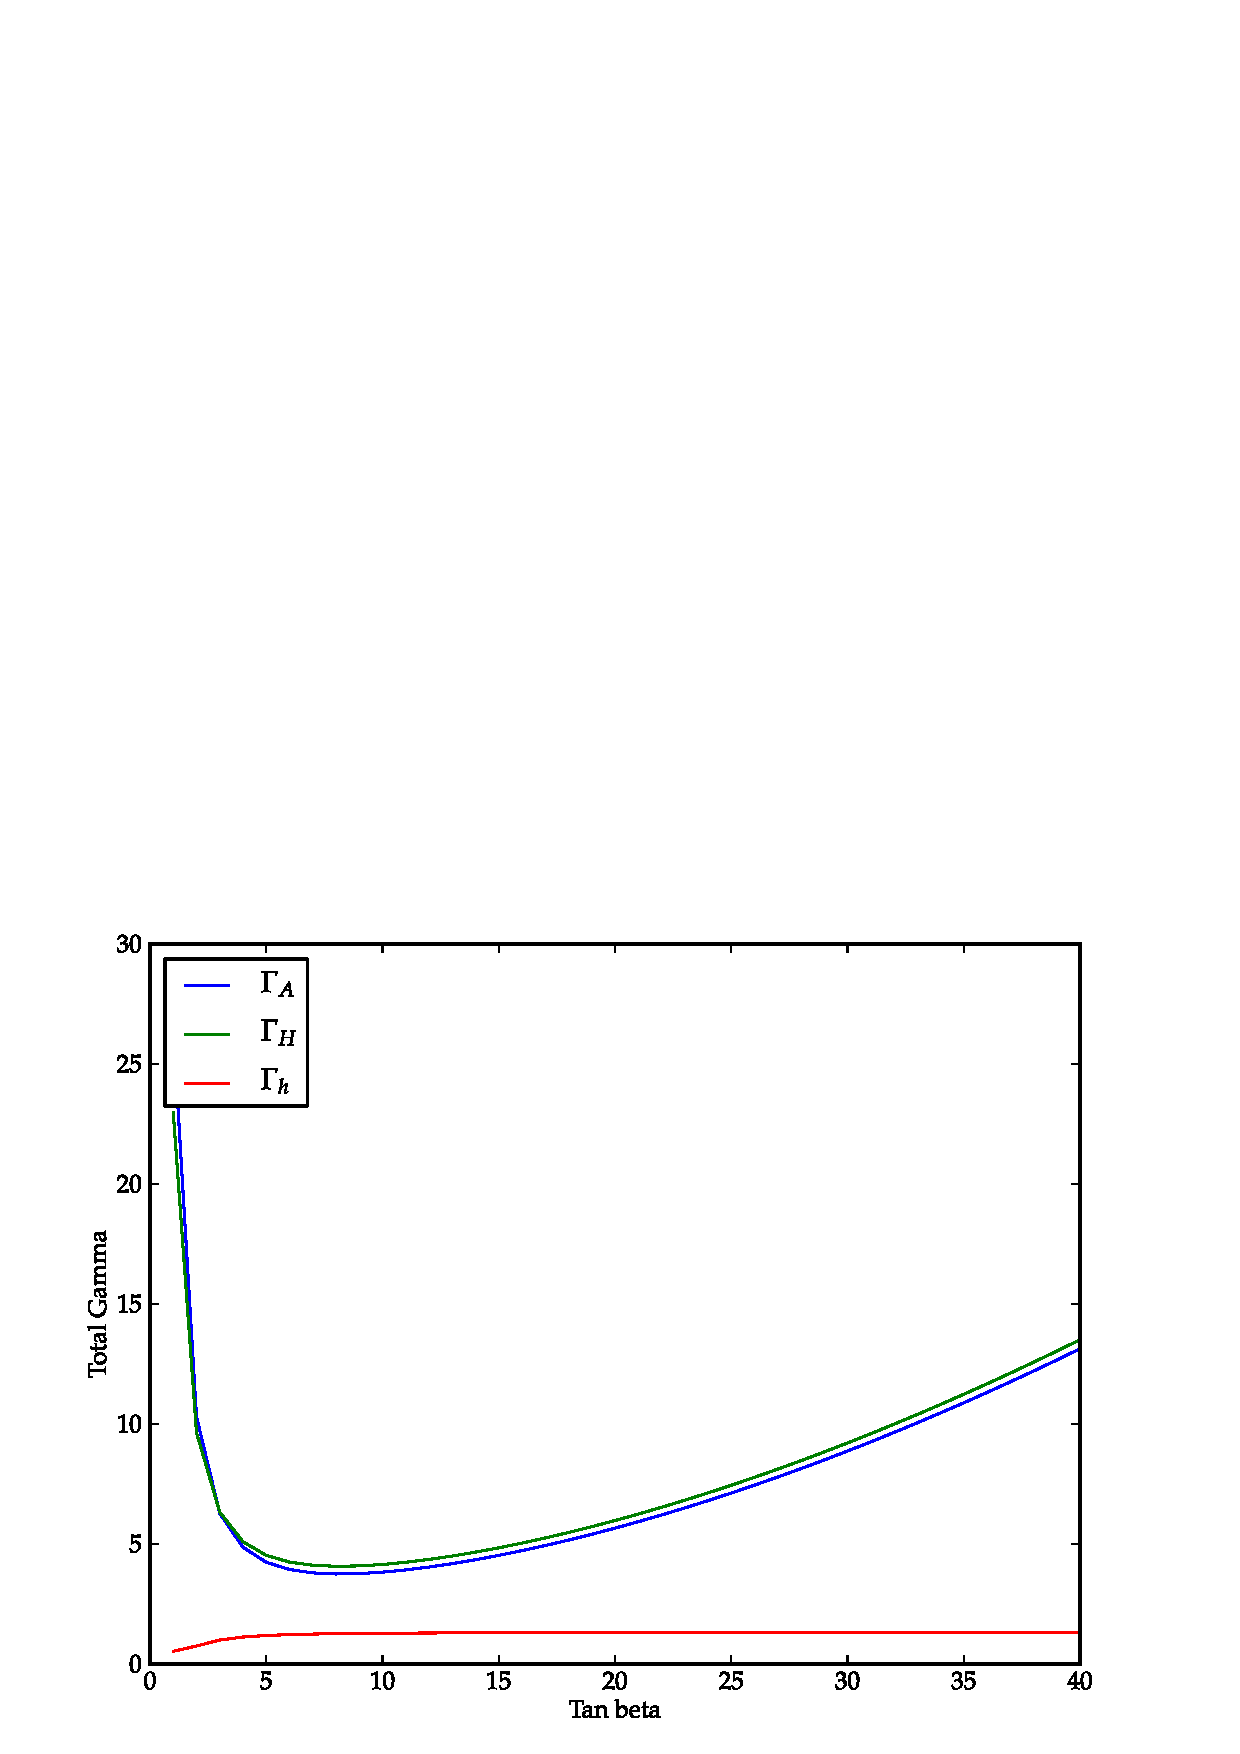
\includegraphics[width=0.7\textwidth]{Theory/figures/TB_gamma.pdf}
	\caption{The inherent width of $A$, $H$, and $h$ as a function of tan$\beta$ when $m_A$=500 GeV. \label{fig:TB_width}}
\end{figure}
%-------------------------------------------------



%\begin{figure}
%	\centering
%	\includegraphics[width=0.7\textwidth]{Theory/figures/mh_max.pdf}
%	\caption{The favored (green) and excluded (red/blue) regions in $m_A/tan\beta$ in the $m_h^{max}$ scenario.  The red regions are excluded by LHC searches, the blue regions by LEP, and the green strip near $tan\beta$=5 is the phase space favored by $m_h$=125.5 GeV.  The fact that the green strip extends across all values of $m_A>$250 GeV means that, in the $m_h^{max}$ scenario, the cross sections of $A$ and $H$ are constrained, but the mass is only minimally restricted. \cite{Carena-2}. \label{fig:mh_max}}
%\end{figure}


\begin{figure}
	\centering
	\includegraphics[width=0.7\textwidth]{Theory/figures/mh_mod.pdf}
	\caption{The favored (green) and excluded (red/blue) regions in 
    $m_A/tan\beta$ in the $m_h^{mod}$ scenario, where the green 
    region shows the phase space that is consistent with $m_h$=126 GeV.  
    After the discovery of $h$ at 126 GeV, the $m_h^{mod}$ 
    scenario is favored because it allows for $m_h$ to have 
    this relatively low value ($m_n^{max}$, on the other 
    hand, pushes $m_h$ more toward 140 GeV).  The 
    left and right plots show the topology for $m_h^{mod+}$ 
    and $m_h^{mod-}$, respectively, the details of which 
    can be found in \cite{Carena-2}. Clearly in this 
    scenario, many values of $m_A$ are open, potentially with large cross-sections. \label{fig:mh_mod}}
\end{figure}





An important and subtle point worth highlighting is that, while 
$A$, $H$, and $H^\pm$ are often called the ``SUSY Higgs bosons'', 
they are SM particles in the sense that they have R-parity of 1.  
The Feynman diagrams for the production of $H$ and $A$ 
in association with $b$-quarks can also be drawn for 
$b$-quark associated production of the SM Higgs boson $h$; 
the most important contribution of SUSY is that, when $tan\beta$ 
is large, it provides an enhancement factor to the vertices that 
drives the production cross section up to a magnitude that could be 
large enough to see in 20 $fb^{-1}$ of proton-proton collisions at $\sqrt{s}$=8 TeV.

However, that does not mean that the SUSY Higgs sector is 
independent of the details of the supersymmetric parameters.  In particular, 
it is possible that H/A decay to a pair of 
SUSY particles, such as charginos or neutralinos.  Depending on the 
scenario, the branching fraction to SUSY particles could be substantial.  
With the large number of free parameters, it is impractical to 
perform a complete scan of the MSSM parameter space, so a 
few benchmark scenarios are chosen where only $m_A$ 
and $tan\beta$ are allowed to vary, and 
the other SUSY parameters are fixed.  The leading benchmark scenario is 
the so-called $m_h^{mod}$ scenario, 
which is an update of the $m_h^{max}$ 
scenario that was used for many years.  In the $m_h^{max}$ 
scenario, the fixed SUSY parameters are assigned values that maximize $m_h$, 
the mass of the light CP-even Higgs.  However, 
in this scenario, $m_h$ is predicted to 
be around 140 GeV, while the experimentally found value is known 
to be around 126 GeV.  In order to reconcile these numbers, 
the updated $m_h^{mod}$ scenario has become 
the more useful benchmark, since it does allow for $m_h$=126 GeV.  
A comparison of the scenarios can be seen in Figures~\ref{fig:mh_max} and ~\ref{fig:mh_mod}.

Other non-MSSM scenarios also have final states with a Higgs boson
decaying to $b$-quarks and produced in association with $b$-quarks,
with cross-sections that could be seen in a few tens of inverse 
femtobarns at the LHC \cite{Gori}.   









\subsection{Constraints on $H/A$}
The discovery in July 2012 of an SM-like Higgs boson provides important constraints of the MSSM Higgs sector,
 but leaves other aspects of the theory tantalizingly unconstrained.  On the one hand, 
for many values of $m_h$, measuring the exact value of $m_h$ 
places a strong constraint on $m_A$--so once $h$ is found, one may have a good idea of what the mass of 
$A$ is, assuming the latter exists.  An important exception is when 
$m_A$ is much larger than the mass of the SM Higgs 
boson $m_h$, which is called the decoupling limit, where the 
properties of $h$ are unaffected by the existence of $H/A$.
  This means that for a light $m_h$ below 140 GeV 
or so (recall that the mass of the discovered particle is about 126 GeV),
 it is very difficult to ascertain constraints on $m_A$ by studying the properties of $h$.  
 As LHC searches advance, though, they constrain our understanding of the BSM 
 Higgs sector from a number of directions: 

\begin{itemize}
    \item Decays of $H/A$ to charginos and neutralinos only occur when kinematically 
allowed--the lack of evidence for these particles (the chargino and neutralino) below several hundred GeV suggests
that in our search region for $H/A$ (which tops out at 800 GeV) there should be little
effect from supersymmetric decays
    \item The chargino and neutralino mass limits also suggest that the higgsino mass
parameter $\mu$ is large, above several hundred GeV
    \item $B_s^0\rightarrow\mu\mu$ appears consistent with the Standard Model predictions,
placing strong constraints on the possibility of nonstandard Higgs contributions
to that decay at loop level \cite{bs_to_mumu}
\end{itemize}

Searches for the charged Higgs bosons, $H^+$ and $H^-$, also provide constraints.
In the MSSM, $H^+$ and $H^-$ are very close to $H$ and $A$ in mass, so searches
for $H^\pm$ can constrain the likely MSSM phase space available for $H$ and $A$ (Figure~\ref{fig:susy_higgs_masses}).
Outside of the MSSM, when some of the assumptions of the MSSM are be relaxed,
it is still possible to have different masses for the heavy Higgs particles.


\begin{figure}
	\centering
	\includegraphics[width=0.7\textwidth]{Theory/figures/susy_higgs_masses.pdf}
	\caption{The mass evolution of the 5 Higgs bosons of the MSSM, with the 
    mass of the Higgs-like indicated by dashed line (126 GeV).  For a large
    range of $h$ masses, the masses of $H$, $A$, and $H^\pm$ evolve very closely
    together, so searches for $H^\pm$ also can provide some indirect constraints
    on the likely masses of $H$ and $A$ \cite{ellis}. 
    \label{fig:susy_higgs_masses}}
\end{figure}
 


\section{From Beautiful Theory to Messy Experiment}

It is the experimentalist's job to understand what all this theoretical physics actually 
looks like it the detector.  This is a deep topic, and one could 
go into great detail, but a few key trends are outlined here.

First, as we've implied throughout this section, many of the particles 
for which a physicist searches cannot be seen directly--they live for a fraction 
of a second, and then decay into other particles.  Those daughter particles often 
decay themselves, and so on into a  multi-step decay chain.  Only 
the particles from the last stage in this chain actually get detected, so part 
of the physicist's job is to reconstruct the original particle(s) 
from the daughter particles.  Once the daughter particles are identified, all that is 
needed to reconstruct the parent particle is the transverse momentum (see below), energy, 
polar angle, and azimuthal angle.  These components go into a Lorentz 4-
vector for each particle, and then the Lorentz-vectors can be added together 
in a relativistically invariant way to get the mass and flight direction of the parent.

Second, certain types of particles leave distinctive signatures.  One important example is that 
particles associated with QCD, quarks and gluons, are subject to the laws of 
QCD confinement.  Once they are produced or excited in the hard scatter, quarks 
and gluons hadronize and shower.  A spray of particles, largely pions, show 
up in the detector in the general direction of the original parent quark or gluon
--if all the shower particles could be collected, they could be recombined into 
the parent particle.  These showers of particles are called jets, and are often 
named after the parent particle, such as $b$-jets, light jets 
and gluon jets.  The topic of jet reconstruction is detailed further in Section~\ref{sec:jet_reco}.  
Photons and electrons shower as well, but they generate much narrower electromagnetic showers that 
are easy to identify and reconstruct, when compared to most QCD showers.  Muons 
have the cleanest signature of all; because of their large mass, they don't 
decay before exiting the detector, so they generally make a single charged track that 
is distinctive in the dedicated muon layers of the detector.

A third important feature of particles as they appear in the detector is their $p_T$, 
or transverse momentum.  Since the initial state of each collision involves two protons, 
which are composite particles, it is impossible to know the exact longitudinal momentum of 
two quarks when they collide.  However, the transverse momentum is zero, so 
in the final state, the transverse momentum must also sum to zero.  When 
heavy particles are created and then decay, or have other particles deflecting off of 
them, the $p_T$ of the resulting particles can be tens 
to hundreds of GeV, which creates a striking signal in the detector and provides 
an experiment handle when trying to understand the event.

The main challenges of this particular search arise from several features of the search.  
First, the final state is all-hadronic, where reconstruction is difficult and 
the QCD background is large.  Second, since the mass of $H$ 
and $A$ are relatively unconstrained, a search has to span a large 
range in $m_A$ in order to be sensitive to discovery.  
Third, the combinatorics of selecting the correct two $b$-jets for reconstruction 
(from the three or more available in an event) require dedicated study.  


\section{Previous Searches}
Searches for $A$ and $H$ in this final state have been performed at the Tevatron
as well as CMS.  The searches at the 
Tevatron were particularly tantalizing because both CDF \cite{CDFbH} and D0 \cite{D0bH} spotted 
slight excesses of events, around 2$\sigma$ standard deviations each, between approximately
100 and 150 GeV.  The LHC experiments (ATLAS and CMS) present an opportunity to
re-examine the same region of phase space, albeit with higher integrated luminosity
and center-of-mass energy.  CMS does not observe an excess in the 100-150 GeV range 
when searching over approximately 5 $fb^{-1}$ of data at $\sqrt{s}$=7 TeV \cite{CMSbH}.

This analysis serves as an important update and extension of the searches done
in other experiments.  Due to differences in the triggers for these analyses,
the ATLAS search does not have access to $m_A$ values below 400 GeV, but it does 
provide the first limits between 400-800 GeV.  This analysis is also the only
search at $\sqrt{s}$=8 TeV, and searches over an integrated luminosity (19.5 $fb^{-1}$)
that is about 4 times higher than the next largest search, done at CMS.


 






